\chapter{Review of the state of the art}

\section{Evolution in internal combustion engines technology and efficiency}
$\frac{HP}{Displacement}$
In this section a review of the key technical improvements occurred to internal combustion engines in the last decades is presented, among with a brief explanation of the current emission limitation rules for both the USA and Europe. The final section will cover the importance of waste heat recovery and why it needs to be researched and adopted in the next years to achieve the planned emissions limitation objectives.

\subsection{Improvements on overall engine efficiency in the last decades}

Since the petroleum crysis of the '70s, an increasing effort on reduction of fuel consumption and increase of power density has begun.

\begin{figure}[ht]
  \centering
  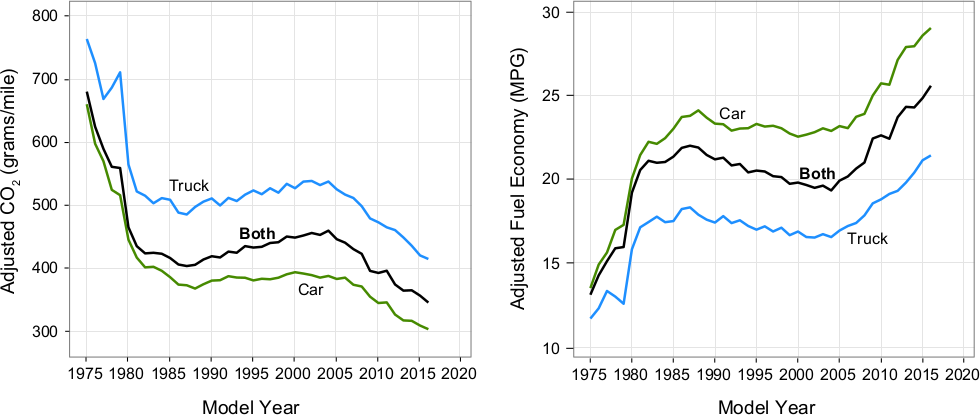
\includegraphics[width=\textwidth]{figures/review/adj_fuel_economy.pdf}
  \caption{Adjusted CO\textsubscript{2} and fuel economy for vehicles model year from 1975 to 2016\label{fig:adj_fuel_economy} }
\end{figure}

As shown in Figure~\ref{fig:adj_fuel_economy}~\cite{EPA2016}, during the last four decades, the fuel consumption and carbon dioxide emissions has been vastly reduced. This great improvement has been possible thanks to some key technical turning points.

One of the main design aspects that have changed significantly over time is how the fuel is delivered into the engine. Until the early 1980s the majority of engines used carburetors to meter fuel delivered to the combustion chamber. More recently, engines with gasoline direct injection (GDI) have begun to replace engines with port fuel injection. GDI equipped engines were first introduced with very limited production in Model Year (MY) 2007. Eight years later GDI engines were installed in about 42 \% of MY 2015 vehicles, and are projected to achieve a 49 \% market share in MY 2016~\cite{EPA2016}.

Another key aspect of engine design that has been vastly improved is the valve-train. The number of valves per cylinder and the ability to alter valve timing during the combustion cycle allowed significant power and efficiency improvements, and nowadays almost the entire fleet of the most relevant car manufacturers has converted to multi-valve design. While some three and five valve engines have been produced, the vast majority of multi-valve engines are based on 4 valves per cylinder~\cite{EPA2016}. In addition to the number of valves per cylinder, designs have evolved that allow engine valves to vary the timing when they are opened or closed with respect to the combustion cycle, creating more flexibility to control engine efficiency, power, and emissions. In Figure~\ref{fig:improvement_valve_fuel_delivery}, the fuel consumption reduction made possible by the improved valve-train and fuel delivery is shown. 

\begin{figure}[ht]
  \centering
  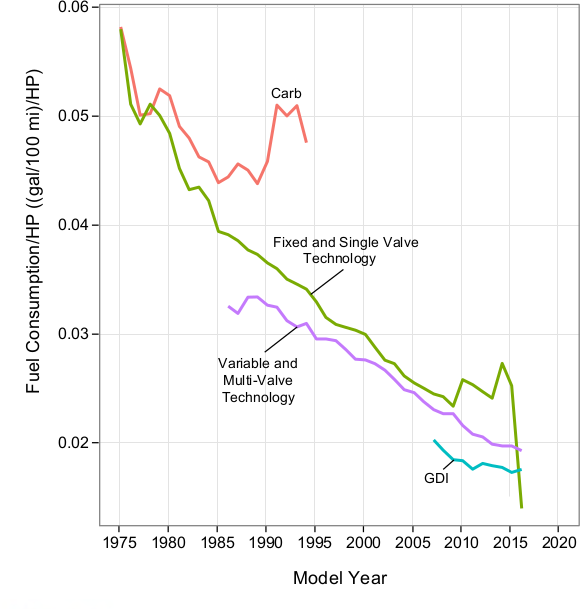
\includegraphics[width=0.6\textwidth]{figures/review/improvement_valve_fuel_delivery.pdf}
  \caption{Trends of fuel consumption variation with the introduction of major fuel delivery and valve-train control technologies \label{fig:improvement_valve_fuel_delivery} }
\end{figure}

As a result of the new fuel delivery systems, along with other reasons, two very noticeable trends in horsepower and displacement delineated. Average horsepower climbed consistently from MY 1982 to MY 2008. Since MY 2008, horsepower trends have been less consistent, and may be beginning to flatten out. From MY 1975 to 1987, the average engine displacement of new vehicles dropped dramatically by nearly 40 \%. From MY 1988 to 2004, displacement generally grew slowly, but the trend reversed in 2005 and engine displacement has been generally decreasing since. In MY 2016, engine displacement is projected to reach the lowest point on record, below the previous lowest average displacement reached in MY 1987~\cite{EPA2016}.

The contrasting trends in horsepower increase and displacement decrease are a proof of the continued improvements in engine design and of the impact of new technologies. The final result is a steady quasi-linear increase of the power density from around 0.5~$\frac{HP}{Displacement}$ in 1975 to around 1.4~$\frac{HP}{Displacement}$ in 2016, with a growth rate of 0.02~$\frac{HP}{in^{2} \cdot year}$. Also the average number of cylinders has gradually reduced.

In Figure~\ref{fig:technology_trends}, a summary of the time trends of the major innovations is reported.

\begin{figure}[ht]
  \centering  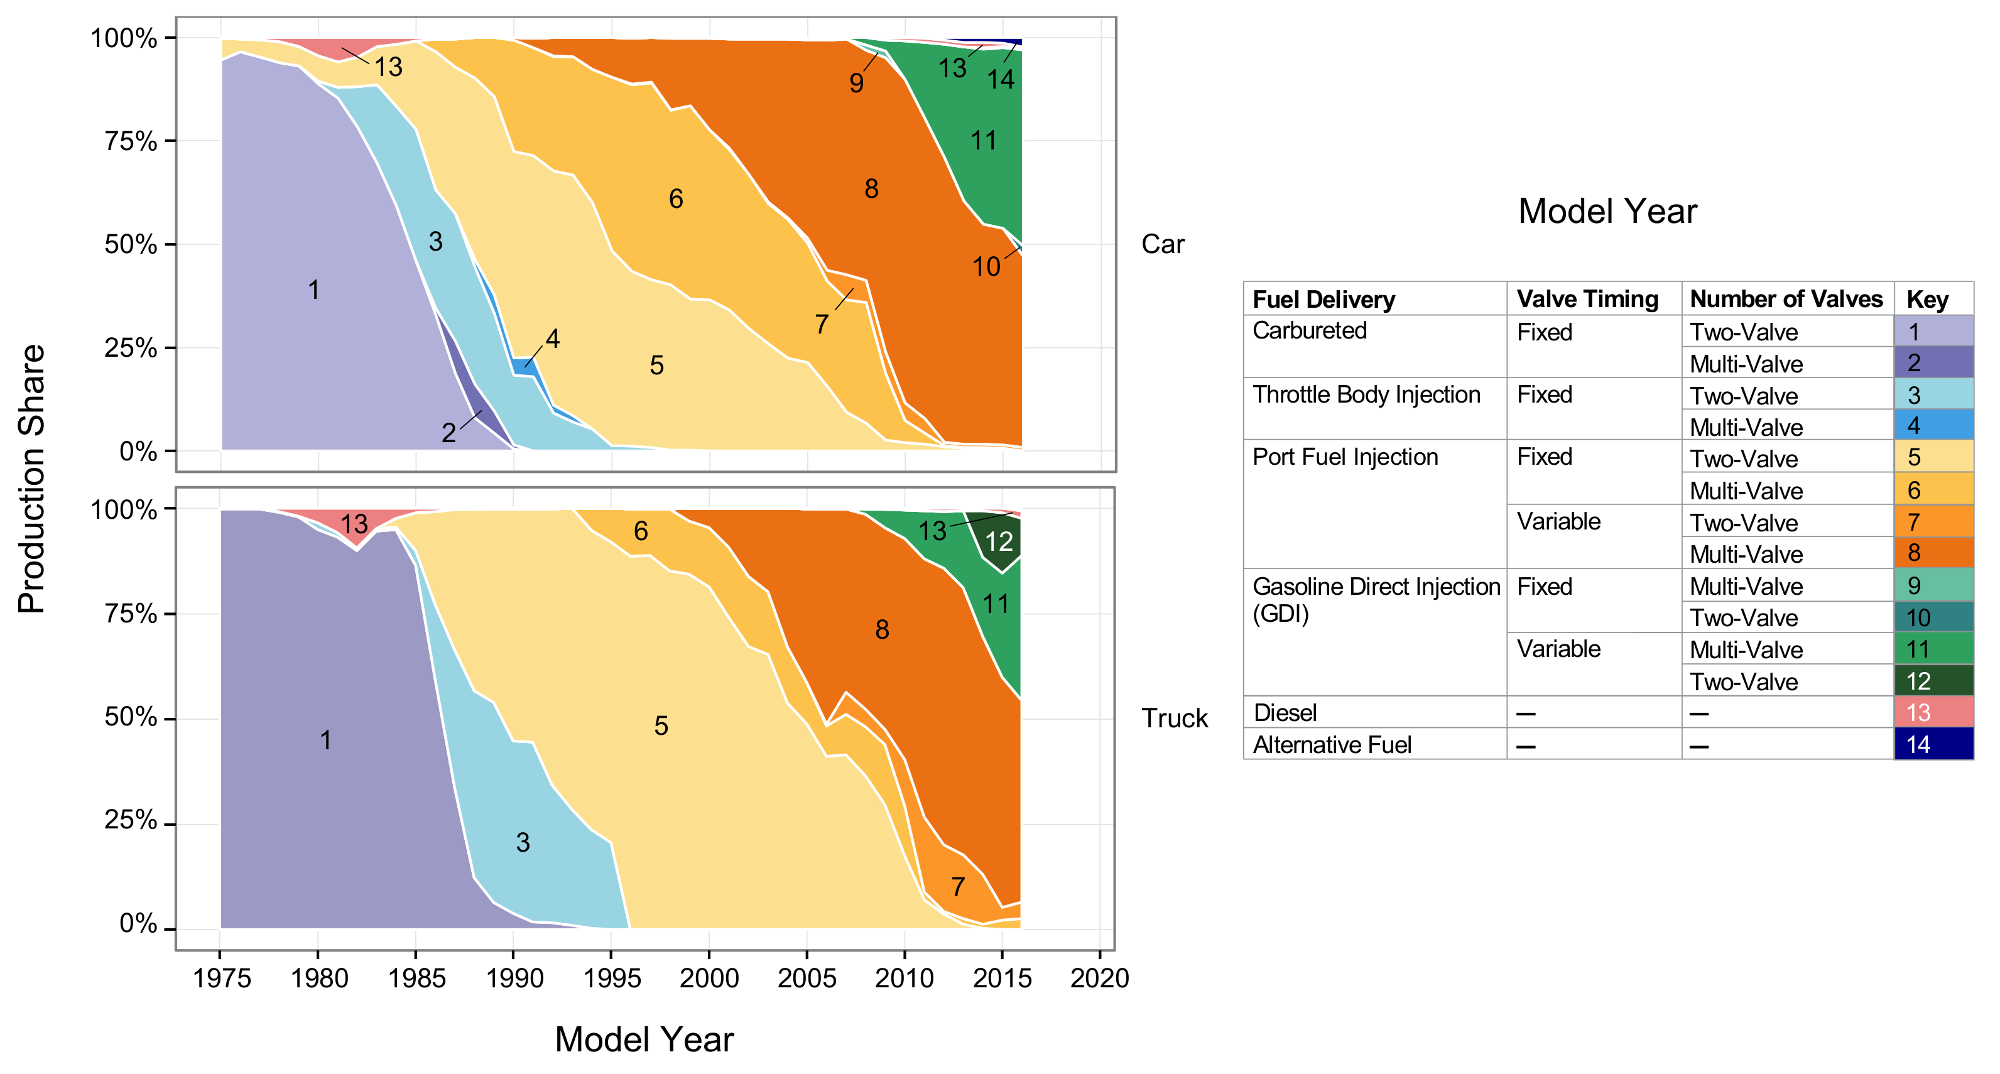
\includegraphics[width=\textwidth]{figures/review/technology_trends.png}
  \caption{Percentage of MY equipped with a certain technology  \label{fig:technology_trends} }
\end{figure}


\subsection{Emission limitations and trends in nowadays technology improvement}
\label{sec:technology_improvements}

Emission limitations are among the main drivers that fostered the continuous strive of greater efficiency in internal combustion engines. In Figure~\ref{fig:emission_standards} a review of the most important emissions standards from across the world, and their Euro equivalence is presented~\cite{Miller2014}. In Figure~\ref{fig:emission_levels} are reported the emission limits for gasoline and diesel powered light vehicles in both the USA and Europe~\cite{Transportpolicy.net2016}.

\begin{figure}[ht]
  \centering
  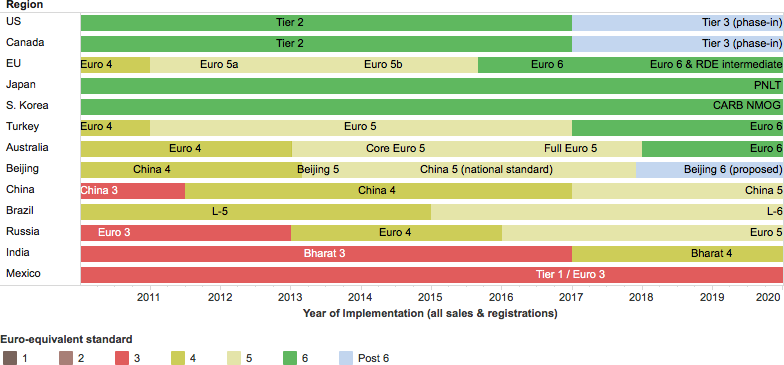
\includegraphics[width=\textwidth]{figures/review/emission_standards.png}
  \caption{Comparison of emissions standards with reference to Euro standards\label{fig:emission_standards} }
\end{figure}

\begin{figure}[ht]
  \centering
  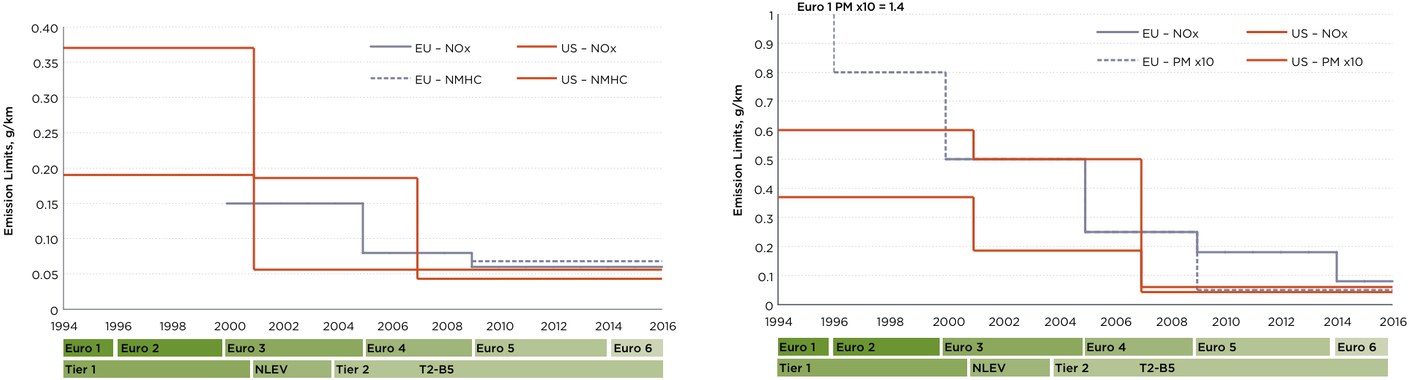
\includegraphics[width=\textwidth]{figures/review/emissions_levels.png}
  \caption{Emissions limits for a) Gasoline and b) Diesel light vehicles in USA and Europe\label{fig:emission_levels} }
\end{figure}

In order to respect the emission standards imposed by current and future rules, the major car manufacturers are adopting some new technologies and some trends are delineating. 

Probably the most noticeable trend in new engines is the \emph{tubo-downsizing}. This new group of engines is characterized usualy by a similar power output with respect to the engine that are replacing, but with a smaller displacement. This result is achieved by the introduction of turbochargers and, often but not always, GDI. Turbo downsized engines are an approach to engine design that provides increased fuel economy by using a smaller engine for most vehicle operation, while retaining the ability to provide more power via the turbocharger, when needed. Turbocharged engines are projected to constitute 22 \% of new vehicle production in 2016, and the penetration trend appears to increase rapidly~\cite{EPA2016}. This is due to the fact the traditionally turbocharged engines were mainly used in high performance vehicles, while now they are being used also on mainstream vehicles. The increased power density and torque made available by the adoption of the turbocharger allows the shifting to designs with fewer cylingers, while the combination with GDI allows a more efficient engine operation and increases the resistance to knocking. In MY 2016, more than 90 \% of new vehicles with gasoline turbocharged engines also use GDI~\cite{EPA2016}. In Figure~\ref{fig:turbodownsizing_distribution}, the distribution of gasoline turbo vehicles is shown. Other new technologies that are gaining traction in the engine design environment are Cylinder Deactivation, Non-Hybrid Stop/Start, and more advanced transmissions, both in form of transmissions with 7 or more gears or Continuous-Variable Transmissions (CVT).

\begin{figure}[ht]
  \centering
  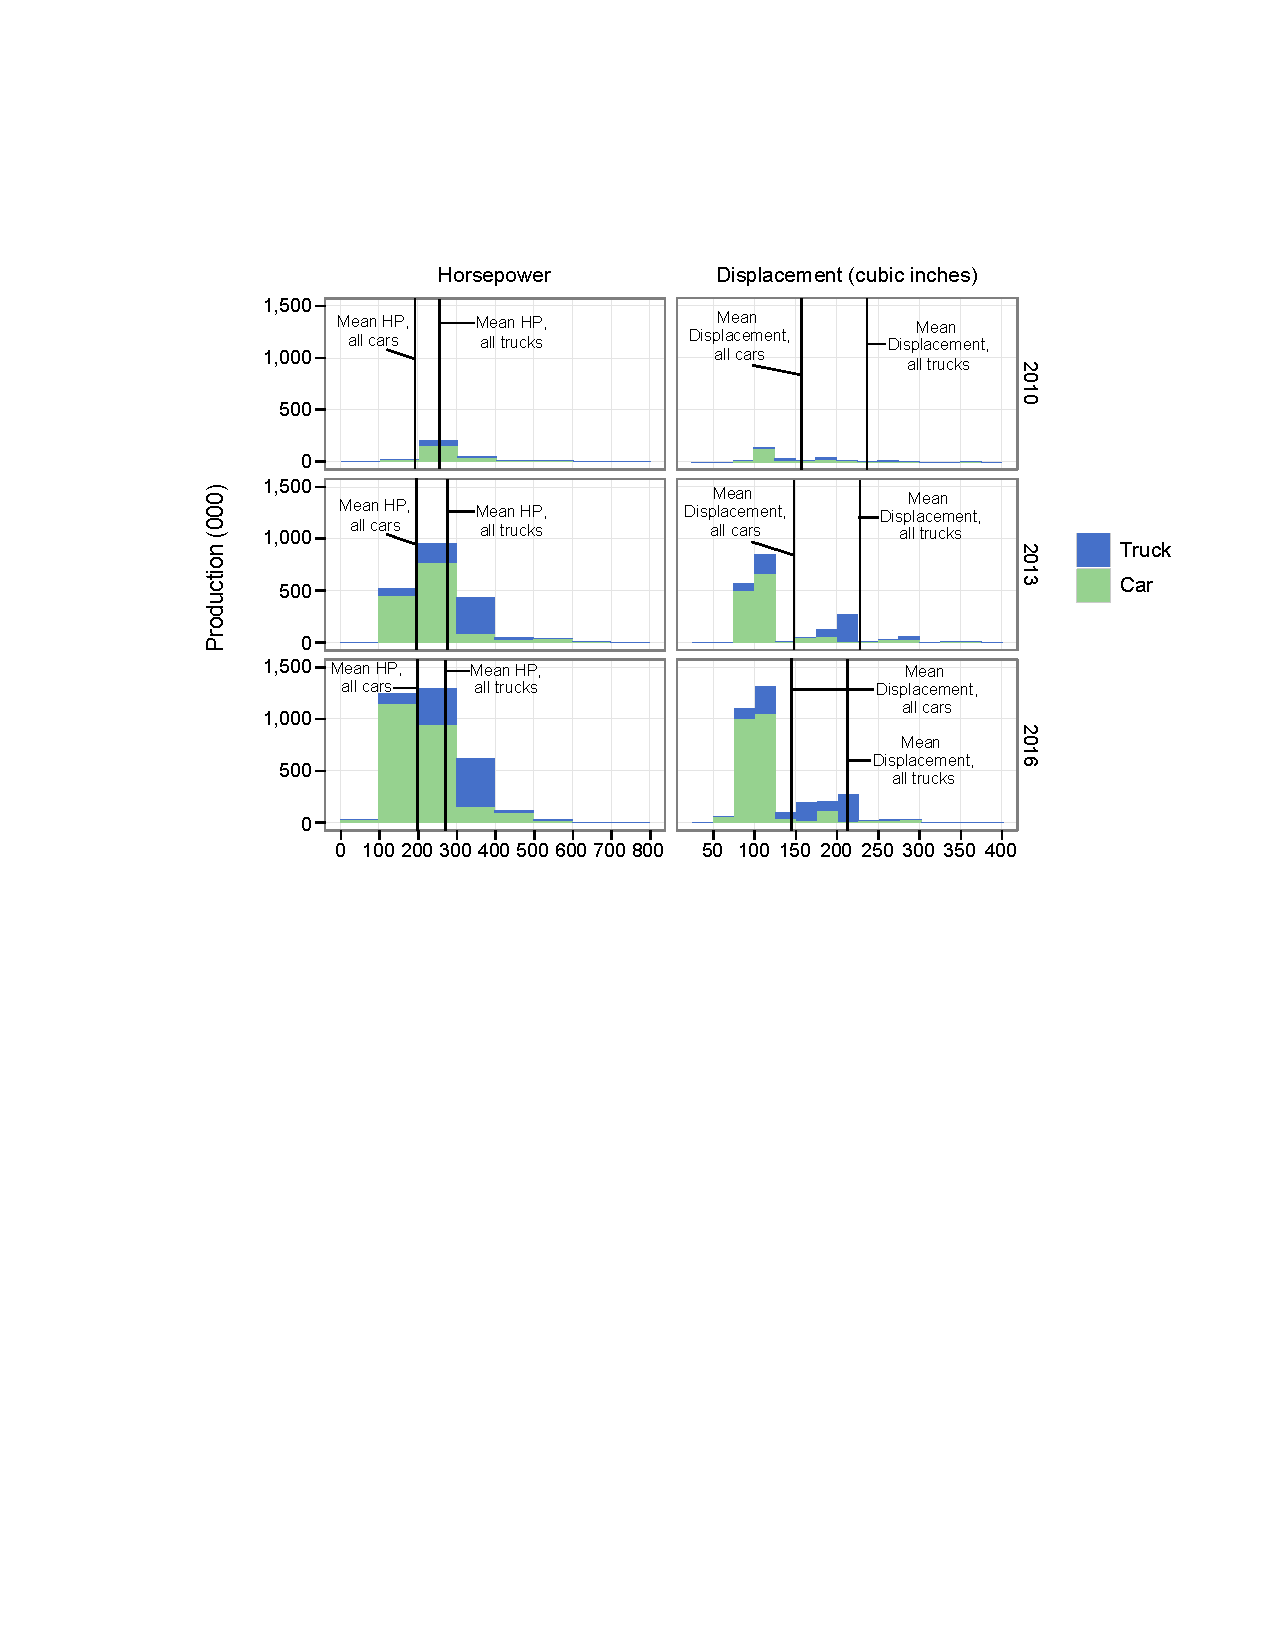
\includegraphics[width=0.8\textwidth]{figures/review/turbodownsizing_distribution.pdf}
  \caption{Distribution of Gasoline Turbo Vehicles by Displacement and Horsepower, MY 2010, 2013, and 2016\label{fig:turbodownsizing_distribution} }
\end{figure}



\emph{Hybrid} vehicle technology is the most diffused technique used to increase the fuel efficiency in ways that transcend the pure ICE efficiency increase. Hybrid vehicles utilize larger battery packs, electric motors, and other components that can  increase vehicle fuel economy. Benefits of hybrids include:
\begin{itemize}
  \item regenerative braking which can capture energy that is otherwise lost in conventional friction braking to charge the battery
  \item availability of two sources of on-board power which can allow the engine to be operated at or  near its peak efficiency more often
  \item shutting off the engine at idle.
\end{itemize} 

Most hybrids provide higher fuel economy than comparable vehicles, although some hybrids have been offered as more performance-oriented vehicles with more minor fuel economy improvements. In Figure~\ref{fig:hybrids} it's shown the distribution in time of the fuel economy between hybrid and non hybrid vehicles, and the historical production of hybrid and electric vehicles.

\begin{figure}[ht]
  \centering
  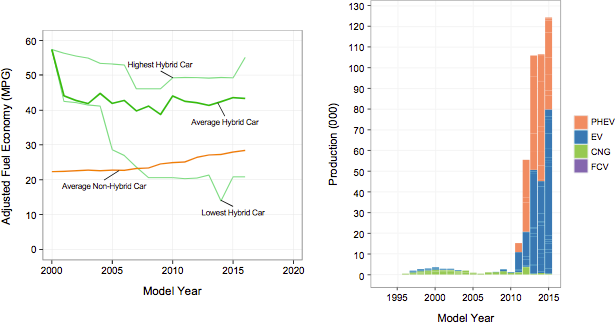
\includegraphics[width=\textwidth]{figures/review/hybrid.png}
  \caption{Comparison fuel economy between non hybrid and hybrid cars and hybrid cars production \label{fig:hybrids} }
\end{figure}


While the average fuel economy of hybrid cars remains higher than the average fuel economy  of non-hybrid cars, the difference appears to be narrowing. Average hybrid car fuel economy  has been relatively stable since MY 2001, while the fuel economy of the average non-hybrid car has increased more than 27 \%. Since MY 2004, the difference in fuel economy between the average hybrid midsize car and the average non-hybrid midsize gasoline car has narrowed from about 25 mpg to about 14 mpg. The primary reason for this trend is continued improvements to the internal combustion engine. Additionally, many technologies introduced or emphasized in early hybrids, such as improved aerodynamics, low rolling resistance tires, and increased use of lightweight materials, have also become more common on non-hybrid vehicles~\cite{EPA2016} .

\subsection{The importance of waste heat recovery}

%%% Local Variables:
%%% mode: latex
%%% TeX-master: "thesis"
%%% End:
